% CVPR 2026 Paper Template; see https://github.com/cvpr-org/author-kit
% Full-length review: built in the template's arXiv mode (page numbers, authors shown).
% For a CVPR submission, switch to [review] and condense to 8 pages.

\documentclass[10pt,twocolumn,letterpaper]{article}

%%%%%%%%% PAPER TYPE
% \usepackage{cvpr}              % To produce the CAMERA-READY version
% \usepackage[review]{cvpr}      % To produce the REVIEW version
\usepackage[pagenumbers]{cvpr} % arXiv version with page numbers

% Import additional packages in the preamble file, before hyperref
%% This file contains a number of tweaks that are typically applied to the main document.
%% They are not enabled by default, but can be enabled by uncommenting the relevant lines.


%%
%% Packages used by this review
%%
\usepackage[T1]{fontenc}
\usepackage{graphicx}
\usepackage{booktabs}
\usepackage{array}
\newcolumntype{L}[1]{>{\raggedright\arraybackslash}p{#1}}
\usepackage{multirow}
\usepackage{amsmath,amssymb}
\usepackage{tikz}
\usetikzlibrary{arrows.meta,positioning,fit,calc,backgrounds}

%%
%% Official support for 2-column teaser figure
%%
\usepackage{cuted} %< for strip environment

%%
%% For auto-referencing of figures (see fig/teaser.tex and \label{} therein) 
%%
\usepackage{currfile} %< for \currfilebase macro

%%
%% caption and (global) spacing overrides
%%
\usepackage{caption} %< for "\captionof" commands (teaser)
% \setlength{\abovecaptionskip}{.5em} % space above caption
% \setlength{\belowcaptionskip}{1em} % space below caption

%%
%% Inline annotations; for predefined colors, refer to "dvipsnames" in the xcolor package:
%% https://tinyurl.com/overleaf-colors
%%
\newcommand{\red}[1]{{\color{red}#1}}
\newcommand{\todo}[1]{{\color{red}#1}}
\newcommand{\TODO}[1]{\textbf{\color{red}[TODO: #1]}}
%%
%% Disable for camera ready / submission by uncommenting these lines:
%%
% \renewcommand{\TODO}[1]{}
% \renewcommand{\todo}[1]{#1}

%%
%% Work harder in optimizing text layout. Typically shrinks text by 1/6 of page, enable
%% it at the very end of the writing process, when you are just above the page limit.
%%
\usepackage{microtype}
\raggedbottom  % do not stretch paragraph spacing to fill columns

%%
%% Fine-tune paragraph spacing.
%%
% \renewcommand{\paragraph}[1]{\vspace{.5em}\noindent\textbf{#1.}}

%%
%% Globally adjusts space between figure and caption.
%%
% \setlength{\abovecaptionskip}{.5em}

%%
%% Allows "the use of \paper to refer to the project name"
%% with automatic management of space at the end of the word.
%%
% \usepackage{xspace}
% \newcommand{\paper}{ProjectName\xspace}

%%
%% Commonly used math definitions.
%%
% \DeclareMathOperator*{\argmin}{arg\,min}
% \DeclareMathOperator*{\argmax}{arg\,max}

%%
%% Tighten underline.
%%
% \usepackage{soul}
% \setuldepth{foobar}

%%
%% Reconfigure paragraph (tweaks spacing)
%%


\definecolor{cvprblue}{rgb}{0.21,0.49,0.74}
\usepackage[pagebackref,breaklinks,colorlinks,allcolors=cvprblue]{hyperref}

\def\paperID{*****}
\def\confName{CVPR}
\def\confYear{2026}

%%%%%%%%% TITLE
\title{Hearing on the Move: A Review of Acoustic Perception\\for Autonomous Intelligent Systems}

%%%%%%%%% AUTHORS
\author{Heena Patel\\
Cyber-Physical Systems Laboratory, Department of ICT and Natural Sciences\\
NTNU - Norwegian University of Science and Technology, \AA{}lesund, Norway\\
{\tt\small heena.s.patel@ntnu.no}
}

\begin{document}
\maketitle
\begin{abstract}
Autonomous systems that hear can detect and locate events that cameras and lidar miss, such as a siren behind a building or a voice under rubble, yet audition remains the least developed sense on robots, drones and vehicles.
This review surveys acoustic perception for these three platform families across six tasks: localization and tracking, event detection, separation and enhancement, joint localization and detection, acoustic mapping, and audio-driven embodied behavior, tracing each from array signal processing to learned, multimodal and language-grounded models.
We argue that one problem sets the field apart from audio on static devices: \emph{ego-noise}, the sound a platform makes itself.
When it dominates, methods that model it explicitly, especially with the platform's own motor or joint state, outperform those that treat it as generic interference.
We review datasets, simulators, toolkits and evaluation protocols, and report reproducible case studies on three public datasets.
On a drone, a learned rotor-noise model raises in-flight localization accuracy within $10^\circ$ from 18\% to 70\%, motor speed helps most when the target is quiet, and the model gives about 10\,dB of beamforming gain.
Across five drones, the tonal share of ego-noise ranges from 1\% to 70\%. The highest values come from drones that were not flying, and rotor-speed variation in flight lowers the tonal share. A learned spatial model removes 6 to 13\,dB on every drone.
On a robot-head array without ego-noise, the same model lowers accuracy for moving talkers. This marks where such models stop helping.
We close with open problems, from hearing at very low signal-to-noise ratios and vibration-referenced noise cancellation to transfer across platforms and privacy.
\end{abstract}

\section{Introduction}
\label{sec:intro}

Sound gives an autonomous system a sense that works around corners, in the dark, through smoke and in every direction at once.
Cameras and lidar need line of sight and a field of view; microphones need neither.
A vehicle can hear another vehicle approaching a blind corner more than a second before a visual detector sees it~\cite{schulz2021hearing}.
A drone can search for a voice it cannot see~\cite{deleforge2019spcup,hoshiba2017uav}.
An embodied agent finds a sounding object in an unexplored house faster when it listens as well as looks~\cite{chen2020soundspaces,gan2020look}, and a robot arm can complete a task inside an opaque bag by listening to the contact~\cite{du2022playitbyear}.

Despite this, hearing remains the least developed sense on most autonomous platforms.
The obstacle is not a lack of methods.
Microphone-array processing is mature~\cite{knapp1976gcc,schmidt1986music,capon1969mvdr}, large pretrained models recognize hundreds of sound classes~\cite{gemmeke2017audioset,kong2020panns,gong2021ast,chen2023beats}, and speech recognition has become robust to many real-world conditions~\cite{radford2023whisper}.
The obstacle is the platform itself.
Robots, drones and vehicles move, vibrate and, above all, make noise.
On a quadrotor, the rotor noise at the drone's own microphones is typically far louder than the sound it is trying to hear~\cite{strauss2018dregon,ruizespitia2018aira}, and on a humanoid, the noise of its own joint motors corrupts what it records whenever it moves~\cite{ince2009template}.

Robot audition emerged as a research field in 2000, when Nakadai \etal proposed \emph{active audition}: a robot that listens while it moves instead of stopping to perceive~\cite{nakadai2000active}.
The field produced the HARK toolkit~\cite{nakadai2017hark}, real-time localization and tracking on mobile robots~\cite{valin2003robust,valin2007tracking}, and later ODAS for embedded hardware~\cite{grondin2022odas}.
Since then, three shifts have changed it.
First, drones became a major platform with an extreme ego-noise problem~\cite{strauss2018dregon,manamperi2022drone,yen2023ncm,chevtchenko2025review}.
Second, learned models moved from niche to default, including joint detection and localization~\cite{adavanne2019seld,shimada2021accdoa,politis2021dcase}.
Third, audio became one input among several to embodied and multimodal intelligence, driven largely by the vision and learning communities~\cite{chen2020soundspaces,gao2020visualechoes,li2022seehearfeel,majumder2021move2hear}.

\paragraph{Relation to prior surveys.}
\Cref{tab:surveys} compares this review with earlier ones.
Two surveys mapped localization for robots up to 2017~\cite{argentieri2015survey,rascon2017review}; Grumiaux \etal reviewed deep learning for localization in rooms~\cite{grumiaux2022survey}; Mesaros \etal gave a tutorial on sound event detection~\cite{mesaros2021tutorial}; and Chevtchenko \etal systematically reviewed drone-based localization, finding that only three of 49 studies implemented real-time on-board localization~\cite{chevtchenko2025review}.
To our knowledge, none treats ego-noise across platforms, covers the embodied and audio-visual work of the vision and learning communities, or links the two.

\begin{table}[t]
\centering
\footnotesize
\setlength{\tabcolsep}{2.6pt}
\begin{tabular}{@{}L{2.55cm}cccccc@{}}
\toprule
Survey & Rob. & Drone & Veh. & Ego-n. & Learn. & Embod. \\
\midrule
Argentieri~\etal~\cite{argentieri2015survey} & \checkmark & & & partial & & \\
Rascon, Meza~\cite{rascon2017review} & \checkmark & & & partial & & \\
Grumiaux~\etal~\cite{grumiaux2022survey} & & & & & \checkmark & \\
Mesaros~\etal~\cite{mesaros2021tutorial} & & & & & \checkmark & \\
Chevtchenko~\etal~\cite{chevtchenko2025review} & & \checkmark & & partial & & \\
\textbf{This review} & \checkmark & \checkmark & \checkmark & \checkmark & \checkmark & \checkmark \\
\bottomrule
\end{tabular}
\caption{Scope of related surveys: platforms (robots, drones, vehicles), treatment of ego-noise, learned methods, and embodied or multimodal learning.}
\label{tab:surveys}
\end{table}

\paragraph{Scope.}
Our scope is acoustic perception on board a moving, self-powered platform; fixed arrays and smart speakers are included only where their methods transfer, and underwater sonar is excluded.

\paragraph{Contributions.}
\begin{enumerate}
\item A task-centered map of the field (\cref{sec:ssl,sec:sed,sec:sep,sec:seld,sec:geometry}) that links classical and learned methods for each task.
\item A cross-platform treatment of ego-noise (\cref{sec:egonoise}) that organizes suppression methods by the information they exploit.
\item A review of audio in embodied, audio-visual and language-grounded intelligence (\cref{sec:embodied}).
\item A guide to datasets, simulators, toolkits (\cref{sec:datasets}) and evaluation protocols (\cref{sec:metrics}).
\item Reproducible case studies on three public datasets (\cref{sec:case}): in-flight localization on a drone, ego-noise structure across five drones, and localization with a robot-head array. Together they quantify when an explicit noise model and motor-speed information help, and when they do not.
\item Open problems with concrete directions (\cref{sec:challenges}).
\end{enumerate}
\Cref{fig:overview} summarizes the structure, and \cref{fig:timeline} places key milestones in time.

\begin{figure*}[t]
\centering
\resizebox{\textwidth}{!}{%
\begin{tikzpicture}[
  font=\footnotesize,
  box/.style={draw=black!60, rounded corners=2pt, align=center, minimum height=0.62cm, text width=2.7cm, fill=white},
  hd/.style={font=\footnotesize\bfseries, align=center, text width=2.9cm},
  grp/.style={draw=black!25, fill=black!3, rounded corners=4pt, inner sep=5pt},
  arr/.style={-{Stealth[length=2mm]}, thick, black!55}]
\node[hd] (h1) at (0,0) {Platform (\S\ref{sec:platforms})};
\node[box, below=0.25cm of h1] (p1) {Ground robots,\\humanoids};
\node[box, below=0.15cm of p1] (p2) {Aerial drones};
\node[box, below=0.15cm of p2] (p3) {Road vehicles};
\node[hd] (h2) at (3.85,0) {Acoustic conditions};
\node[box, below=0.25cm of h2] (c1) {Ego-noise (\S\ref{sec:egonoise})};
\node[box, below=0.15cm of c1] (c2) {Motion of array\\and sources};
\node[box, below=0.15cm of c2] (c3) {Wind, reverberation,\\compute};
\node[hd] (h3) at (7.7,0) {Tasks};
\node[box, below=0.25cm of h3] (t1) {Localization, tracking\\(\S\ref{sec:ssl})};
\node[box, below=0.15cm of t1] (t2) {Event detection (\S\ref{sec:sed})};
\node[box, below=0.15cm of t2] (t3) {Separation,\\enhancement (\S\ref{sec:sep})};
\node[box, below=0.15cm of t3] (t4) {Joint SELD (\S\ref{sec:seld})};
\node[box, below=0.15cm of t4] (t5) {Mapping, geometry\\(\S\ref{sec:geometry})};
\node[hd] (h4) at (11.55,0) {Embodied use (\S\ref{sec:embodied})};
\node[box, below=0.25cm of h4] (u1) {Navigation to sound};
\node[box, below=0.15cm of u1] (u2) {Occluded hazard\\detection};
\node[box, below=0.15cm of u2] (u3) {Search and rescue};
\node[box, below=0.15cm of u3] (u4) {Manipulation,\\interaction};
\node[hd] (h5) at (15.4,0) {Side information};
\node[box, below=0.25cm of h5] (s1) {Motor, joint state};
\node[box, below=0.15cm of s1] (s2) {IMU, vibration};
\node[box, below=0.15cm of s2] (s3) {Vision, depth};
\node[box, below=0.15cm of s3] (s4) {Language};
\begin{scope}[on background layer]
\node[grp, fit=(h1)(p3)] (g1) {};
\node[grp, fit=(h2)(c3)] (g2) {};
\node[grp, fit=(h3)(t5)] (g3) {};
\node[grp, fit=(h4)(u4)] (g4) {};
\node[grp, fit=(h5)(s4)] (g5) {};
\end{scope}
\draw[arr] (g1.east |- p2) -- (g2.west |- p2);
\draw[arr] (g2.east |- c2) -- (g3.west |- c2);
\draw[arr] (g3.east |- t2) -- (g4.west |- t2);
\draw[arr] (g5.south) |- node[pos=0.75, below, font=\scriptsize, black!70] {informs ego-noise models and multimodal fusion} ($(g3.south)+(0.6,-0.45)$) -- ($(g3.south)+(0.6,0)$);
\end{tikzpicture}}
\caption{Structure of the review. A platform sets the acoustic conditions, of which ego-noise is the most severe. Perception tasks turn microphone signals into events, directions and geometry that embodied agents act on. Side information that only an autonomous platform has (its own motor, motion and visual state) can inform ego-noise models and multimodal fusion.}
\label{fig:overview}
\end{figure*}

\begin{figure*}[t]
\centering
\resizebox{\textwidth}{!}{%
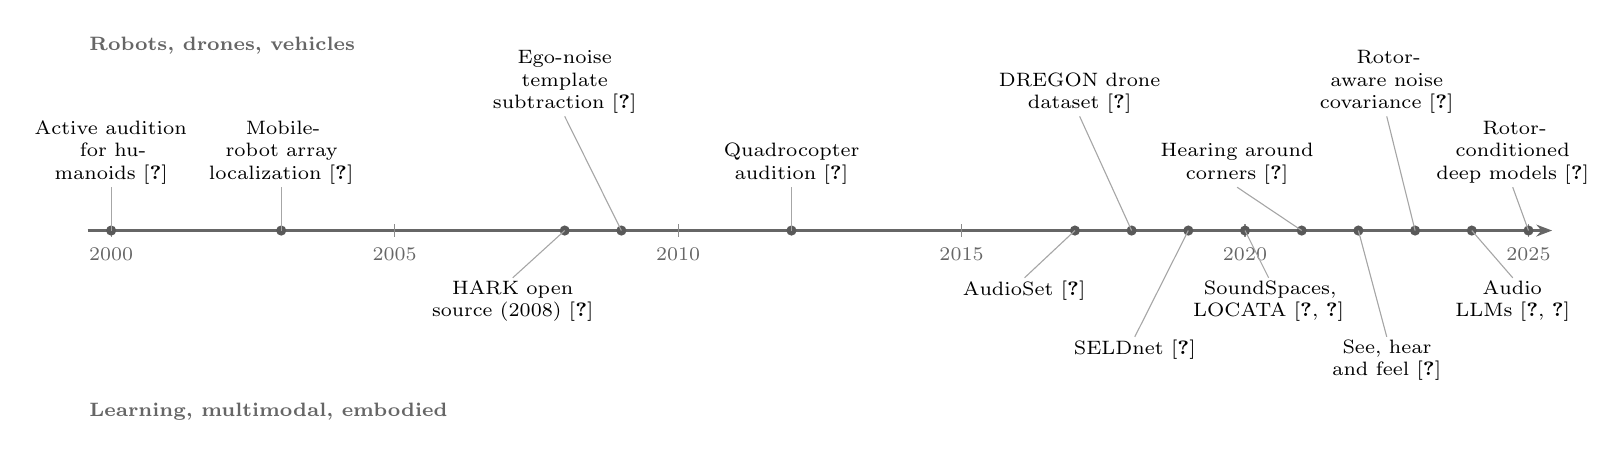
\begin{tikzpicture}[font=\scriptsize,
  ev/.style={align=center, text width=2.05cm, inner sep=1pt},
  dot/.style={circle, fill=black!65, inner sep=1.3pt}]
\draw[-{Stealth[length=2mm]}, thick, black!60] (0,0) -- (18.6,0);
% x = (year - 2000) * 0.72 + 0.3
\foreach \y/\lab in {2000/2000, 2005/2005, 2010/2010, 2015/2015, 2020/2020, 2025/2025}
  { \pgfmathsetmacro{\x}{(\y-2000)*0.72+0.3} \draw[black!45] (\x,-0.08) -- (\x,0.08); \node[below, black!60] at (\x,-0.1) {\lab}; }
% above the axis: robots and drones
\node[dot] at (0.30,0) {}; \node[ev, above] at (0.30,0.55) {Active audition\\for humanoids~\cite{nakadai2000active}}; \draw[black!35] (0.30,0) -- (0.30,0.55);
\node[dot] at (2.46,0) {}; \node[ev, above] at (2.46,0.55) {Mobile-robot array\\localization~\cite{valin2003robust}}; \draw[black!35] (2.46,0) -- (2.46,0.55);
\node[dot] at (6.78,0) {}; \node[ev, above] at (6.06,1.45) {Ego-noise template\\subtraction~\cite{ince2009template}}; \draw[black!35] (6.78,0) -- (6.06,1.45);
\node[dot] at (8.94,0) {}; \node[ev, above] at (8.94,0.55) {Quadrocopter\\audition~\cite{okutani2012quadrocopter}}; \draw[black!35] (8.94,0) -- (8.94,0.55);
\node[dot] at (13.26,0) {}; \node[ev, above] at (12.6,1.45) {DREGON drone\\dataset~\cite{strauss2018dregon}}; \draw[black!35] (13.26,0) -- (12.6,1.45);
\node[dot] at (15.42,0) {}; \node[ev, above] at (14.6,0.55) {Hearing around\\corners~\cite{schulz2021hearing}}; \draw[black!35] (15.42,0) -- (14.6,0.55);
\node[dot] at (16.86,0) {}; \node[ev, above] at (16.5,1.45) {Rotor-aware noise\\covariance~\cite{yen2023ncm}}; \draw[black!35] (16.86,0) -- (16.5,1.45);
\node[dot] at (18.30,0) {}; \node[ev, above] at (18.1,0.55) {Rotor-conditioned\\deep models~\cite{gulli2025rotor}}; \draw[black!35] (18.30,0) -- (18.1,0.55);
% below the axis: learning and embodied
\node[dot] at (6.06,0) {}; \node[ev, below] at (5.4,-0.6) {HARK open\\source (2008)~\cite{nakadai2017hark}}; \draw[black!35] (6.06,0) -- (5.4,-0.6);
\node[dot] at (12.54,0) {}; \node[ev, below] at (11.9,-0.6) {AudioSet~\cite{gemmeke2017audioset}}; \draw[black!35] (12.54,0) -- (11.9,-0.6);
\node[dot] at (13.98,0) {}; \node[ev, below] at (13.3,-1.35) {SELDnet~\cite{adavanne2019seld}}; \draw[black!35] (13.98,0) -- (13.3,-1.35);
\node[dot] at (14.70,0) {}; \node[ev, below] at (15.0,-0.6) {SoundSpaces,\\LOCATA~\cite{chen2020soundspaces,evers2020locata}}; \draw[black!35] (14.70,0) -- (15.0,-0.6);
\node[dot] at (16.14,0) {}; \node[ev, below] at (16.5,-1.35) {See, hear\\and feel~\cite{li2022seehearfeel}}; \draw[black!35] (16.14,0) -- (16.5,-1.35);
\node[dot] at (17.58,0) {}; \node[ev, below] at (18.1,-0.6) {Audio LLMs~\cite{gong2024ltu,tang2024salmonn}}; \draw[black!35] (17.58,0) -- (18.1,-0.6);
\node[font=\scriptsize\bfseries, black!60, anchor=west] at (-0.1,2.35) {Robots, drones, vehicles};
\node[font=\scriptsize\bfseries, black!60, anchor=west] at (-0.1,-2.3) {Learning, multimodal, embodied};
\end{tikzpicture}}
\caption{Selected milestones in acoustic perception for autonomous systems. Above the axis: platform-centered robot, drone and vehicle audition. Below: learning, audio-visual and embodied work. Positions follow the publication year.}
\label{fig:timeline}
\end{figure*}

\section{Background and Problem Formulation}
\label{sec:background}

\paragraph{Signal model.}
An array of $M$ microphones at positions $\mathbf{r}_1,\dots,\mathbf{r}_M$ observes, in the short-time Fourier transform (STFT) domain,
\begin{equation}
\mathbf{x}(f,t) = \sum_{k=1}^{K} \mathbf{a}(f,\mathbf{u}_k)\, s_k(f,t) + \mathbf{n}_{\text{ego}}(f,t) + \mathbf{n}_{\text{env}}(f,t),
\label{eq:model}
\end{equation}
where $s_k$ are $K$ target sources, $\mathbf{n}_{\text{ego}}$ is the noise the platform makes itself, and $\mathbf{n}_{\text{env}}$ is environmental noise and reverberation.
For a far-field source from unit direction $\mathbf{u}$, the steering vector is
\begin{equation}
\mathbf{a}(f,\mathbf{u}) = \big[e^{\,j2\pi f\,\mathbf{r}_1^{\top}\mathbf{u}/c},\dots,e^{\,j2\pi f\,\mathbf{r}_M^{\top}\mathbf{u}/c}\big]^{\top},
\label{eq:steer}
\end{equation}
with $c$ the speed of sound.
Spatial covariances $\mathbf{R}_x(f)=\mathbb{E}[\mathbf{x}\mathbf{x}^{H}]$ and $\mathbf{R}_n(f)$ for the noise summarize the second-order statistics that most classical methods use.

\paragraph{What makes autonomous platforms different.}
Three properties of \cref{eq:model} distinguish autonomous platforms from static devices.
First, $\mathbf{n}_{\text{ego}}$ is often the dominant term, so the signal-to-noise ratio (SNR) at the microphones is strongly negative~\cite{strauss2018dregon,ruizespitia2018aira}.
Second, the array moves, so $\mathbf{u}_k$ changes over time even for static sources, and reverberation changes as the platform moves through a space.
Third, $\mathbf{n}_{\text{ego}}$ is a function of the platform's own state, such as rotor speeds or joint velocities, which the platform knows.

\paragraph{Binaural hearing.}
Two-microphone robots, such as humanoid heads, rely on interaural time and level differences, as human hearing does.
They suffer from front-back ambiguity, which head movement can resolve~\cite{ma2017binaural}; this was one of the original motivations for active audition~\cite{nakadai2000active}.

\paragraph{Tasks.}
We use the following task definitions.
\emph{Localization} estimates the direction (and sometimes distance) of each source; \emph{tracking} links estimates over time.
\emph{Sound event detection} (SED) estimates which classes are active and when~\cite{mesaros2021tutorial}.
\emph{Separation and enhancement} recover the target signals $s_k$.
\emph{Sound event localization and detection} (SELD) estimates class, activity and direction jointly~\cite{adavanne2019seld}.
\emph{Acoustic mapping} recovers the positions of sources, of the platform, or of the surrounding geometry.

\section{Platforms and Their Acoustic Conditions}
\label{sec:platforms}

The same algorithm can succeed on a smart speaker and fail on a drone, because the platform decides what the microphones hear.
\Cref{tab:platforms} compares the three platform families along the dimensions that matter most.

\paragraph{Ground robots and humanoids.}
Robot audition grew out of humanoid robotics, where the goal was natural interaction: localizing and separating several talkers and recognizing their speech~\cite{nakadai2000active,nakadai2017hark}.
Mobile robots added real-time localization and tracking with on-board arrays~\cite{valin2003robust,valin2007tracking,grondin2019lightweight}.
Arrays are small (a head or a torso), the robot often moves, and the dominant ego-noise comes from fans and from joint motors that switch on and off with each gesture or step~\cite{ince2009template,schmidt2016dictionary}.
Because a robot knows its own joint state, this noise is partly predictable, which has made robots the proving ground for motor-informed ego-noise suppression~\cite{ince2009template,schmidt2018egonoise,schmidt2019informed}.
Robot manipulators increasingly use sound as a contact sensor, for example to estimate liquid height while pouring~\cite{liang2019pouring} or to act inside occluded containers~\cite{du2022playitbyear}.

\paragraph{Aerial drones.}
Drones are the hardest case.
Microphones sit tens of centimeters from rotors spinning thousands of times per minute, and the rotor noise combines strong harmonics of each rotor's shaft rate with broadband aerodynamic noise~\cite{strauss2018dregon,yen2023ncm}.
Recordings of drone ego-noise have very low SNR, change with the drone's maneuvers, and are highly correlated across microphones~\cite{ruizespitia2018aira}.
Drone audition is motivated mainly by search and rescue: 82\% of the 49 studies in a recent systematic review target this use~\cite{chevtchenko2025review}, and fielded systems have localized voices from the air in outdoor demonstrations~\cite{hoshiba2017uav}.
Early work localized sources outdoors with an array embedded in a quadrocopter~\cite{okutani2012quadrocopter} and learned the rotor-noise correlation matrix to suppress it~\cite{furukawa2013ncm}.
Public datasets now provide on-board recordings with ground truth~\cite{strauss2018dregon,wang2019avq,ruizespitia2018aira}.
Payload and power budgets limit both the array and the on-board compute.

\paragraph{Road vehicles.}
Vehicles use sound mainly for safety: detecting emergency vehicles and hazards that are not yet visible.
Early work modeled the urban soundscape to detect horns and sirens as anomalies~\cite{marchegiani2017urban}, and later work localized and classified sirens from stereo recordings by segmenting spectrograms~\cite{marchegiani2022sirens}.
A roof-mounted array can detect a vehicle approaching a blind corner from reflections off nearby walls, before it enters line of sight~\cite{schulz2021hearing}, and even two low-cost microphones can detect sirens and estimate their direction~\cite{sun2021siren}.
Self-supervised learning from stereo sound has been used to track moving vehicles, with a visual network as teacher~\cite{gan2019stereo}.
The main noise sources are the vehicle's own engine and tires and, at speed, wind at the microphones.

\begin{table}[t]
\centering
\footnotesize
\setlength{\tabcolsep}{3pt}
\begin{tabular}{@{}L{1.55cm}L{2.0cm}L{2.0cm}L{2.0cm}@{}}
\toprule
 & Ground robots & Drones & Vehicles \\
\midrule
Main use & interaction, speech, manipulation & search and rescue & safety, occlusion \\
Ego-noise & fans, joint motors & rotors (tonal and broadband) & engine, tires, wind \\
Noise varies with & joint motion & rotor speed & speed, road \\
Side info & joint state & motor speed, IMU & speed, CAN data \\
Array size & head or torso & limited by payload & roof, large \\
Key refs & \cite{nakadai2000active,valin2007tracking,ince2009template,schmidt2018egonoise} & \cite{strauss2018dregon,furukawa2013ncm,yen2023ncm,hoshiba2017uav} & \cite{schulz2021hearing,marchegiani2017urban,marchegiani2022sirens,gan2019stereo} \\
\bottomrule
\end{tabular}
\caption{Acoustic conditions on the three platform families. In every case the platform's own state carries information about its noise, which static devices do not have.}
\label{tab:platforms}
\end{table}

\section{Sound Source Localization and Tracking}
\label{sec:ssl}

Localization is the most studied task in robot audition and the one most affected by ego-noise.
\Cref{tab:ssl} summarizes representative methods.

\subsection{Classical methods}
Generalized cross-correlation with phase transform (GCC-PHAT) estimates the time delay between each pair of microphones~\cite{knapp1976gcc}.
Steered response power with phase transform (SRP-PHAT) sums these correlations over all pairs for every candidate direction and picks the maximum~\cite{dibiase2000srp}.
Subspace methods such as MUSIC~\cite{schmidt1986music} split $\mathbf{R}_x(f)$ into signal and noise subspaces and search for steering vectors (\cref{eq:steer}) orthogonal to the latter.
Both assume that noise is spatially white, which ego-noise is not (\cref{sec:egonoise}).
Generalized eigenvalue decomposition MUSIC (GEVD-MUSIC) removes this assumption by whitening with a noise covariance $\mathbf{R}_n(f)$, solving
\begin{equation}
\mathbf{R}_x(f)\,\mathbf{e} = \lambda\, \mathbf{R}_n(f)\,\mathbf{e};
\label{eq:gevd}
\end{equation}
it improved robot localization robustness by 5 to 6\,dB SNR~\cite{nakamura2011gevd} and became the basis of drone audition~\cite{okutani2012quadrocopter,furukawa2013ncm}.

On mobile robots, Valin \etal localized sources with an eight-microphone array in real time~\cite{valin2003robust} and then combined a frequency-domain steered beamformer with a particle filter to track several moving sources over about 7\,m~\cite{valin2007tracking}.
Later work reduced the cost of SRP-PHAT by coarse-to-fine scanning and tracked directions with a modified Kalman filter, using up to four and thirty times less computation respectively~\cite{grondin2019lightweight}; these methods underlie the ODAS toolkit~\cite{grondin2022odas}.

\subsection{Binaural and active localization}
Two-microphone systems use interaural cues.
Deep networks that map the full cross-correlation function and interaural level differences to azimuth, combined with head rotation to resolve front-back confusions, localize multiple sources robustly in reverberant rooms~\cite{ma2017binaural}.
More generally, an agent can move to hear better: active audition listens during motion rather than in stop-perceive-act cycles~\cite{nakadai2000active}, and Move2Hear learns where to move to improve source separation~\cite{majumder2021move2hear}.

\subsection{Learned methods}
Neural localizers learn the map from multichannel features (phase maps, GCC features, SRP maps or raw spectrograms) to directions, by classification over a grid or by regression.
A convolutional network trained on noise signals generalizes to speech~\cite{chakrabarty2017doa}; deep networks localize and detect multiple speakers from a robot~\cite{he2018multispeaker}; and Cross3D tracks a source in strongly reverberant rooms by running a causal 3D convolutional network over SRP-PHAT maps, trained on simulated trajectories and evaluated on real LOCATA recordings~\cite{diazguerra2021cross3d}.
Grumiaux \etal survey this literature in depth~\cite{grumiaux2022survey}.
On drones, a neural time-frequency mask that suppresses ego-noise before SRP-based or spatial-filtering localization outperforms either component alone~\cite{wang2022drone}, and a TDOA-based method with noise angular spectrum subtraction works at low signal-to-drone-noise ratios on an irregular on-board array~\cite{manamperi2022drone}.

\subsection{Tracking}
Moving platforms need temporally consistent estimates.
Particle filters~\cite{valin2007tracking} and Kalman filters~\cite{grondin2019lightweight} link frame-wise estimates and suppress isolated errors.
The LOCATA challenge benchmarks localization and tracking from single static sources up to multiple moving sources observed by a moving array~\cite{evers2020locata}.

\begin{table}[t]
\centering
\footnotesize
\setlength{\tabcolsep}{2.4pt}
\begin{tabular}{@{}L{2.5cm}L{1.3cm}L{1.85cm}L{1.45cm}@{}}
\toprule
Method & Venue & Key idea & Platform \\
\midrule
GCC-PHAT~\cite{knapp1976gcc} & TASSP'76 & pairwise delay & any \\
SRP-PHAT~\cite{dibiase2000srp} & thesis'00 & steered power & any \\
MUSIC~\cite{schmidt1986music} & TAP'86 & signal subspace & any \\
Active audition~\cite{nakadai2000active} & AAAI'00 & listen while moving & humanoid \\
Valin \etal~\cite{valin2007tracking} & RAS'07 & beamformer + particle filter & mobile robot \\
GEVD-MUSIC~\cite{nakamura2011gevd} & IROS'11 & noise whitening & robot \\
Okutani \etal~\cite{okutani2012quadrocopter} & IROS'12 & GEVD on a quadrocopter & drone \\
Chakrabarty, Habets~\cite{chakrabarty2017doa} & WASPAA \mbox{'17} & CNN on phase & static \\
Ma \etal~\cite{ma2017binaural} & TASLP'17 & DNN + head motion & binaural head \\
He \etal~\cite{he2018multispeaker} & ICRA'18 & DNN, multi-speaker & robot \\
Cross3D~\cite{diazguerra2021cross3d} & TASLP'21 & 3D CNN on SRP maps & static \\
Wang, Cavallaro~\cite{wang2022drone} & Sens.\,J'22 & DNN mask + SRP & drone \\
Manamperi \etal~\cite{manamperi2022drone} & TASLP'22 & TDOA + noise subtraction & drone \\
\bottomrule
\end{tabular}
\caption{Representative sound source localization methods, ordered from classical to learned.}
\label{tab:ssl}
\end{table}

\section{Sound Event Detection and Classification}
\label{sec:sed}

Detection answers \emph{what} is sounding and \emph{when}; Mesaros \etal give a tutorial treatment of the task, its methods and its evaluation~\cite{mesaros2021tutorial}.

\paragraph{Data.}
Large labeled collections made modern detectors possible.
ESC-50 provides 2{,}000 five-second clips over 50 environmental classes~\cite{piczak2015esc}; AudioSet provides a sound-event ontology and about two million human-labeled 10-second clips from web video~\cite{gemmeke2017audioset}; FSD50K provides over 51k openly licensed clips labeled with 200 AudioSet classes~\cite{fonseca2022fsd50k}; and VGGSound provides about 200k web videos whose audio and visual content correspond~\cite{chen2020vggsound}.

\paragraph{Models.}
Pretrained audio neural networks (PANNs) trained on AudioSet transfer well to downstream tasks~\cite{kong2020panns}.
The Audio Spectrogram Transformer (AST) showed that a convolution-free, attention-only model reaches state-of-the-art accuracy, 0.485 mAP on AudioSet~\cite{gong2021ast}.
BEATs learns general audio representations by self-supervised prediction of discrete labels from an acoustic tokenizer~\cite{chen2023beats}.
Contrastive language-audio pretraining (CLAP) aligns audio with text and enables zero-shot classification of classes never seen in training~\cite{elizalde2023clap}.

\paragraph{On autonomous platforms.}
These models are trained on clean web audio, while a platform hears targets at low SNR under its own noise; domain shift is therefore the central challenge.
Vehicle work has addressed it with task-specific pipelines: modeling the urban soundscape to detect anomalous alerting sounds and then classifying them~\cite{marchegiani2017urban}, treating spectrograms as images to segment sirens from background noise before classifying and localizing them~\cite{marchegiani2022sirens}, and detecting sirens and their direction with only two low-cost microphones~\cite{sun2021siren}.
Robot manipulators use detection-style models to infer physical state from sound, for example liquid height during pouring~\cite{liang2019pouring}.
Few of these systems have been tested under the strong ego-noise of drones, and we are not aware of a public benchmark for multi-class event detection on board a drone.

\section{Separation, Enhancement and Speech}
\label{sec:sep}

Separation recovers the target signal itself, for recognition or for a human operator.

\paragraph{Spatial filtering.}
The minimum variance distortionless response (MVDR) beamformer~\cite{capon1969mvdr} keeps the target direction undistorted and minimizes everything else:
\begin{equation}
\mathbf{w}_{\text{MVDR}}(f)=\frac{\mathbf{R}_n^{-1}(f)\,\mathbf{a}(f,\mathbf{u})}{\mathbf{a}^{H}(f,\mathbf{u})\,\mathbf{R}_n^{-1}(f)\,\mathbf{a}(f,\mathbf{u})}.
\label{eq:mvdr}
\end{equation}
Like GEVD-MUSIC (\cref{eq:gevd}), it needs the noise covariance $\mathbf{R}_n$, which is exactly what an ego-noise model provides.
Neural mask estimation made such beamformers practical without explicit noise recordings: a network estimates time-frequency masks for speech and noise, which yield the covariances that define the beamformer~\cite{heymann2016mask}.

\paragraph{Learned separation.}
Supervised separation with deep networks covers speech enhancement, multi-talker separation and dereverberation~\cite{wang2018overview}.
Conv-TasNet works directly on waveforms and surpassed ideal time-frequency masks on speech separation~\cite{luo2019convtasnet}.
Separation quality is now usually reported as scale-invariant signal-to-distortion ratio (SI-SDR), introduced because the earlier SDR could be misleading~\cite{leroux2019sisdr}.

\paragraph{Audio-visual separation.}
Vision tells a separator which source to extract.
The Sound of Pixels separates sources by the image regions that produce them~\cite{zhao2018pixels}; multisensory features learned from synchronization separate on-screen from off-screen sound~\cite{owens2018multisensory}; Looking to Listen isolates a chosen speaker from a crowd using the speaker's face~\cite{ephrat2018looking}; and audio-visual object embeddings learned without labels support separation, localization and active-speaker detection~\cite{afouras2020avobjects}.
An agent can also move to improve separation: Move2Hear learns camera and microphone motion that maximizes predicted separation quality~\cite{majumder2021move2hear}.

\paragraph{On drones.}
Drone speech enhancement must cope with ego-noise far louder than speech.
Neural masks estimated by a single-channel network suppress ego-noise before spatial processing~\cite{wang2022drone}; audio-visual recordings from a quadcopter provide baselines for localization and enhancement~\cite{wang2019avq}; and conditioning end-to-end enhancement networks on rotor speed improves speech recovery~\cite{gulli2025rotor}.

\paragraph{Speech recognition.}
For human-robot interaction, enhancement is usually followed by recognition.
Large weakly supervised models such as Whisper, trained on 680{,}000 hours of transcribed audio, generalize zero-shot to many conditions~\cite{radford2023whisper}, but their robustness to strong ego-noise has not been characterized.

\section{Joint Sound Event Localization and Detection}
\label{sec:seld}

Sound event localization and detection (SELD) estimates class, activity and direction together, which is the natural output format for an autonomous system that must know both what is happening and where.

\paragraph{Methods.}
SELDnet, a convolutional recurrent network, introduced joint detection and direction-of-arrival regression for overlapping sources~\cite{adavanne2019seld}.
The activity-coupled Cartesian DOA (ACCDOA) representation merged the two outputs into a single vector per class, whose length encodes activity and whose direction encodes the source direction~\cite{shimada2021accdoa}.
Event-independent networks assign overlapping events to separate output tracks~\cite{cao2021einv2}.

\paragraph{Evaluation.}
The first SELD evaluation, run in DCASE 2019, ranked systems by localization and detection scored separately; joint metrics that require an event to be both correctly detected and close to its true direction changed the ranking of several systems~\cite{politis2021dcase}.
STARSS23 provides real recordings with spatiotemporal annotations together with 360-degree video, and shows that visual cues reduce localization error~\cite{shimada2023starss23}.

\paragraph{Gap.}
All SELD benchmarks so far use static arrays without ego-noise.
Moving SELD to robots and drones requires both new data and methods that model the platform's own noise.

\section{Ego-Noise: The Defining Problem}
\label{sec:egonoise}

Ego-noise is the sound a platform makes itself.
It differs from the interference that room acoustics and audio benchmarks assume in four ways.
It is \emph{loud}: on drones, targets are routinely recorded at strongly negative SNR~\cite{strauss2018dregon,deleforge2019spcup,ruizespitia2018aira}, and in our drone case study localization breaks down between $-10$ and $-20$\,dB (\cref{sec:case-dregon}).
It is \emph{close and fixed}: its sources sit at known places on the body, so it has strong spatial structure, and drone ego-noise is highly correlated across microphones~\cite{ruizespitia2018aira}.
It is \emph{non-stationary}: it changes with every gesture, maneuver or acceleration.
And it is \emph{partly predictable}, because the platform knows its own motor and joint state.
The last property is what an autonomous platform has that a static device does not, and the most effective methods exploit it.

\paragraph{Structure of rotor and motor noise.}
A rotor turning at $f_0$ revolutions per second produces tones at multiples of $f_0$, strongest at multiples of the blade passing frequency $B f_0$ for $B$ blades, plus broadband aerodynamic noise; both shift with speed~\cite{yen2023ncm}.
Robot joint motors produce harmonic noise whose structure follows motor speed~\cite{schmidt2018egonoise}.
Our case studies confirm and qualify both points on real drone data: predicted rotor tones follow the measured motor speed closely, yet on most drones the noise is largely broadband, and the share of energy in tones ranges from 1\% to 70\% across five drones (\cref{sec:case-drones}), so frequency-domain masking alone cannot remove it.

\paragraph{A taxonomy of suppression methods.}
We group ego-noise methods by the information they exploit (\cref{tab:egonoise}).

\emph{(i) Spatial noise models.}
Because ego-noise sources are fixed relative to the array, their spatial covariance $\mathbf{R}_n(f)$ can be learned from noise-only recordings and used to whiten the observations, as in GEVD-MUSIC~\cite{nakamura2011gevd,okutani2012quadrocopter} or MVDR (\cref{eq:mvdr}).
Furukawa \etal estimated the noise correlation matrix for a multirotor drone and showed that it improves localization~\cite{furukawa2013ncm}.

\emph{(ii) State-informed models.}
The platform's own state predicts its noise.
On robots, template subtraction selects a pre-recorded noise template from the current joint status~\cite{ince2009template}, and motor data can guide or regularize multichannel dictionaries of ego-noise~\cite{schmidt2016dictionary,schmidt2018egonoise,schmidt2019informed}.
On drones, rotor-noise-aware covariance estimation combines a multi-sensory estimate of rotor noise power with a model of the acoustic paths from rotors to microphones, and reports up to about 28\,dB rotor-noise reduction on in-flight recordings~\cite{yen2023ncm}.

\emph{(iii) Learned suppression.}
Neural networks estimate time-frequency masks that remove ego-noise before localization~\cite{wang2022drone}, in the spirit of mask-based beamforming~\cite{heymann2016mask}, or are conditioned directly on rotor speed for end-to-end enhancement~\cite{gulli2025rotor}.
These methods can capture non-linear structure that covariance models miss, but they need training data from the same platform.

\emph{(iv) Reference sensors.}
Accelerometers or other vibration sensors close to the noise sources can, in principle, provide a reference signal with phase, which would allow tones to be subtracted rather than masked.
This direction is largely open for autonomous platforms; flight-controller IMUs are usually logged at rates too low to capture the acoustic band (\cref{sec:case-dregon}).

\begin{table}[t]
\centering
\footnotesize
\setlength{\tabcolsep}{3pt}
\begin{tabular}{@{}L{1.75cm}L{2.15cm}L{1.65cm}L{1.9cm}@{}}
\toprule
Approach & Information used & Platforms & Refs \\
\midrule
Spatial noise model & noise-only recordings & robots, drones & \cite{nakamura2011gevd,okutani2012quadrocopter,furukawa2013ncm} \\
State-informed & joint or motor state & robots, drones & \cite{ince2009template,schmidt2016dictionary,schmidt2018egonoise,schmidt2019informed,yen2023ncm} \\
Learned & paired training data & drones & \cite{wang2022drone,gulli2025rotor} \\
Reference sensors & vibration with phase & open & -- \\
\bottomrule
\end{tabular}
\caption{Ego-noise suppression grouped by the information it exploits. Methods further down use more platform-specific information and need more platform-specific data.}
\label{tab:egonoise}
\end{table}

\paragraph{Vehicles.}
Ego-noise on road vehicles is less studied in the perception literature.
Engine and tire noise are partly predictable from vehicle speed and engine state, and wind noise grows with speed; the occluded-vehicle detector of Schulz \etal reports its headline accuracy with a static ego-vehicle~\cite{schulz2021hearing}.
Transferring state-informed ego-noise models from robots and drones to vehicles is a clear gap.

\paragraph{Real-time constraints.}
Ego-noise suppression must run on the platform.
Only three of 49 drone localization studies in a recent systematic review ran in real time on board~\cite{chevtchenko2025review}, which makes efficient methods~\cite{grondin2019lightweight,grondin2022odas} as important as accurate ones.

\section{Acoustic Mapping, Echoes and Geometry}
\label{sec:geometry}

Sound also reveals the space around a platform, which matters most when vision is degraded.

\paragraph{Mapping from sources.}
Acoustic SLAM jointly estimates the trajectory of a moving array and a map of the surrounding sources from direction-of-arrival measurements~\cite{evers2018slam}.

\paragraph{Active echoes.}
A platform that emits sound can infer geometry from the echoes.
BatVision predicts depth and spatial layout from binaural recordings of emitted chirps~\cite{christensen2020batvision}, and VisualEchoes learns spatial image representations through echolocation, which transfer to depth estimation and navigation~\cite{gao2020visualechoes}.

\paragraph{Geometry from ambient and binaural sound.}
Audio-visual floorplan reconstruction uses sound to infer the layout of rooms the camera has not seen~\cite{purushwalkam2021floorplan}.
Binaural recordings can predict the semantic segmentation and depth of the surrounding scene and can be super-resolved spatially~\cite{vasudevan2020binaural}, and video can turn mono audio into binaural audio by exploiting the visible scene layout~\cite{gao2019visualsound}.

\paragraph{Acoustic rendering.}
Neural acoustic fields learn a continuous model of how sound propagates between any emitter and listener position in a scene~\cite{luo2022naf}.
Visual acoustic matching re-renders a recording to sound as if it were made in the room shown in an image~\cite{chen2022vam}, and novel-view acoustic synthesis predicts what a scene sounds like from a new viewpoint~\cite{chen2023nvas}.
These models give an agent an internal model of room acoustics, which could in turn support prediction of what it should hear and hence anomaly detection.

\section{Audio in Embodied and Multimodal Intelligence}
\label{sec:embodied}

Much of the recent progress in machine hearing for agents has come from the vision and learning communities, where sound is treated as one modality of an embodied agent rather than as a signal to be cleaned.
\Cref{tab:embodied} summarizes representative work.

\paragraph{Audio-visual navigation.}
SoundSpaces introduced navigation to a sounding target in realistic scanned 3D environments, with audio rendered by geometric acoustic simulation, and showed that audio improves embodied navigation~\cite{chen2020soundspaces}.
Gan \etal proposed a parallel formulation with a visual mapper, a sound-localization module and a planner~\cite{gan2020look}.
Follow-up work learned to set waypoints with an acoustic memory~\cite{chen2021waypoints}, extended the task to semantically meaningful sounding objects~\cite{chen2021semantic}, and to moving sound sources amid distracting noise~\cite{younes2023catch}.
Simulation platforms have matured: SoundSpaces~2.0 renders continuous, configurable acoustics for visual-acoustic learning~\cite{chen2022soundspaces2}, and Sonicverse provides a multisensory household simulator for agents that see and hear~\cite{gao2023sonicverse}.
These platforms make large-scale training possible, but they usually omit the agent's own ego-noise, which \cref{sec:egonoise,sec:case} show is the dominant difficulty on real platforms.

\paragraph{Self-supervised audio-visual learning.}
Correspondence between sight and sound is a strong free supervisory signal.
Ambient sound supervises visual representation learning~\cite{owens2016ambient}; audio-visual correspondence localizes sounding objects in images~\cite{arandjelovic2018objects,senocak2018localize}; audio-visual events can be localized in time in unconstrained video~\cite{tian2018ave}; and audio-visual objects can be discovered and tracked from unlabeled video~\cite{afouras2020avobjects}.
For autonomous vehicles, a visual network has served as teacher for tracking vehicles from stereo sound~\cite{gan2019stereo}, and binaural recordings have been used to predict semantic segmentation and depth~\cite{vasudevan2020binaural}.
Sound can also detect what vision cannot yet see: an acoustic detector anticipated vehicles behind blind corners more than a second before a visual detector reached the same accuracy~\cite{schulz2021hearing}.

\paragraph{Manipulation and interaction.}
Audio carries contact information.
Fusing vision, audio from a contact microphone, and touch improves robotic manipulation on dense packing and pouring~\cite{li2022seehearfeel}; audio estimates liquid height during pouring~\cite{liang2019pouring}; audio helps imitation learning when the scene is visually occluded, reaching 70\% success on extracting keys from a bag, which the authors report is 50\% higher than a policy without audio~\cite{du2022playitbyear}; and object-centric datasets pair visual, auditory and tactile representations of the same objects~\cite{gao2021objectfolder}.

\paragraph{Audio and language.}
Contrastive language-audio pretraining links sounds to text and enables zero-shot classification~\cite{elizalde2023clap}.
Audio language models now cast audio tasks as text generation~\cite{deshmukh2023pengi}, and perceive and reason about general sounds, speech and music~\cite{gong2024ltu,tang2024salmonn}.
For autonomous systems, these models promise open-vocabulary event detection and natural-language reports of what the platform hears.
Their robustness to ego-noise and their latency on embedded hardware are, as far as we are aware, untested.

\begin{table}[t]
\centering
\footnotesize
\setlength{\tabcolsep}{2.4pt}
\begin{tabular}{@{}L{2.25cm}L{1.3cm}L{2.0cm}L{1.45cm}@{}}
\toprule
Work & Venue & Contribution & Setting \\
\midrule
SoundSpaces~\cite{chen2020soundspaces} & ECCV'20 & audio-visual navigation & simulation \\
Gan \etal~\cite{gan2020look} & ICRA'20 & mapper + sound + planner & simulation \\
Waypoints~\cite{chen2021waypoints} & ICLR'21 & acoustic memory & simulation \\
Semantic AV-Nav~\cite{chen2021semantic} & CVPR'21 & semantic sounding goals & simulation \\
Move2Hear~\cite{majumder2021move2hear} & ICCV'21 & move to separate & simulation \\
SoundSpaces 2.0~\cite{chen2022soundspaces2} & NeurIPS'22 & continuous acoustics & simulation \\
Catch me if you hear me~\cite{younes2023catch} & RA-L'23 & moving sound sources & simulation \\
Sonicverse~\cite{gao2023sonicverse} & ICRA'23 & multisensory household & simulation \\
See, Hear, Feel~\cite{li2022seehearfeel} & CoRL'22 & vision, audio, touch & real robot \\
Play it by Ear~\cite{du2022playitbyear} & RSS'22 & audio under occlusion & real robot \\
Hearing around corners~\cite{schulz2021hearing} & RA-L'21 & occluded vehicles & real vehicle \\
\bottomrule
\end{tabular}
\caption{Representative embodied and multimodal work that uses sound. Most audio-visual navigation is still developed in simulation without ego-noise.}
\label{tab:embodied}
\end{table}

\section{Datasets, Simulators and Toolkits}
\label{sec:datasets}

Progress in acoustic perception for autonomous systems is limited less by models than by data recorded on real platforms.
\Cref{tab:datasets} lists the main public resources and what each can test.

\begin{table*}[t]
\centering
\footnotesize
\setlength{\tabcolsep}{3pt}
\begin{tabular}{@{}L{3.1cm}L{2.0cm}L{1.3cm}L{1.4cm}L{7.6cm}@{}}
\toprule
Resource & Platform & Real ego-noise & Ground truth & What it tests \\
\midrule
DREGON~\cite{strauss2018dregon} & drone, 8 mics & yes & motion capture & in-flight localization; per-rotor speed and IMU logged \\
SP Cup 2019~\cite{deleforge2019spcup} & drone & yes & yes & localization for search and rescue \\
SP Cup ego-noise~\cite{deleforge2019spcup} & 10 drones, 1--16 mics & yes & -- & ego-noise of different drones; used in \cref{sec:case} \\
AIRA-UAS~\cite{ruizespitia2018aira} & drone & yes & -- & ego-noise during maneuvers and from nearby drones \\
AVQ~\cite{wang2019avq} & drone, 8 mics + camera & yes & from video & audio-visual localization, tracking and enhancement outdoors \\
LOCATA~\cite{lollmann2018locata,evers2020locata} & robot head (12 mics), spherical, planar, hearing aids; static and moving & no & motion capture & localization and tracking of moving talkers in a reverberant room; used in \cref{sec:case} \\
OVAD~\cite{schulz2021hearing} & vehicle, 56 mics & partly & yes & detection of occluded vehicles \\
STARSS23~\cite{shimada2023starss23} & static array + 360$^\circ$ video & no & motion capture & audio-visual SELD in real rooms \\
AudioSet~\cite{gemmeke2017audioset} & web video & no & labels & event classification and pretraining \\
ESC-50~\cite{piczak2015esc} & curated clips & no & labels & environmental sound classification \\
FSD50K~\cite{fonseca2022fsd50k} & curated clips & no & labels & open event classification \\
VGGSound~\cite{chen2020vggsound} & web video & no & labels & audio-visual recognition \\
\midrule
SoundSpaces~\cite{chen2020soundspaces,chen2022soundspaces2} & simulator & no & exact & audio-visual navigation and rendering \\
Sonicverse~\cite{gao2023sonicverse} & simulator & no & exact & multisensory household agents \\
ObjectFolder~\cite{gao2021objectfolder} & object models & no & exact & visual, auditory and tactile object properties \\
\midrule
HARK~\cite{nakadai2017hark} & toolkit & -- & -- & robot localization, separation, recognition \\
ODAS~\cite{grondin2022odas} & toolkit & -- & -- & embedded localization, tracking, separation \\
\bottomrule
\end{tabular}
\caption{Public datasets, simulators and toolkits. Only DREGON combines real ego-noise with the platform's own motor state and ground-truth directions; none yet combines a moving platform, real ego-noise, platform state, high-rate vibration sensing, multiple sound classes and video.}
\label{tab:datasets}
\end{table*}

Three gaps stand out.
First, the benchmarks with rich annotations (STARSS23 for SELD, SoundSpaces for navigation, AudioSet for classification) do not include ego-noise, while the datasets that do (DREGON, AIRA-UAS, AVQ) are small and focus on localization and enhancement.
Second, no public benchmark yet combines a moving platform, real ego-noise, the platform's state, high-rate vibration sensing, multiple sound classes and visual input.
Such a benchmark would let the embodied-learning and robot-audition communities measure progress on the same problem.
Third, availability is fragile: of the ten drone ego-noise sets released with the SP Cup, two could no longer be downloaded at the time of writing, so archival hosting with persistent identifiers matters as much as collection.
Toolkits such as HARK and ODAS lower the barrier to real-time deployment, but they implement classical pipelines and would benefit from integration with learned models.

\section{Evaluation Protocols and Metrics}
\label{sec:metrics}

Results across the field are hard to compare because tasks, metrics and test conditions vary.
\Cref{tab:metrics} lists the metrics in common use.

\begin{table}[t]
\centering
\footnotesize
\setlength{\tabcolsep}{2.6pt}
\begin{tabular}{@{}L{1.6cm}L{4.25cm}L{1.55cm}@{}}
\toprule
Task & Metrics & Refs \\
\midrule
Localization & angular error (mean, median); accuracy within a threshold, \eg $10^\circ$ & \cite{evers2020locata,grumiaux2022survey} \\
Tracking & localization metrics over time; track continuity and swaps & \cite{evers2020locata} \\
Event detection & segment- or event-based F-score and error rate & \cite{mesaros2021tutorial} \\
SELD & location-aware detection plus class-aware localization error & \cite{politis2021dcase} \\
Separation & SI-SDR & \cite{leroux2019sisdr} \\
Speech & word error rate & \cite{radford2023whisper} \\
Navigation & success rate; success weighted by path length & \cite{chen2020soundspaces} \\
\bottomrule
\end{tabular}
\caption{Common evaluation metrics by task.}
\label{tab:metrics}
\end{table}

\paragraph{Recommendations.}
Five practices would make results on autonomous platforms more comparable.
\emph{(i) Report SNR at the microphones}, measured or controlled, rather than only the source level; performance on drones depends far more on SNR than on method details (\cref{sec:case-dregon}).
\emph{(ii) Separate noise-model data from test data}: when a method learns an ego-noise model, it should be learned from recordings disjoint from the test signals, as in the held-out protocol of our drone case study (\cref{sec:case-dregon}).
\emph{(iii) Fix frame alignment independently of the methods compared}: array and ground-truth frames should be aligned once, on separate data, with a method not under test.
\emph{(iv) Report per-condition results}, such as per flight or per SNR, since averages can hide where a method helps most; in our drone case study the benefit of motor-speed information is concentrated in the quiet-source condition.
\emph{(v) Report a baseline without a noise model and the noise conditions}, because a noise model can also cost accuracy when the SNR is high and the noise close to diffuse, as on the robot-head array of \cref{sec:case-locata}.

\section{Case Studies on Public Datasets}
\label{sec:case}

To test the argument of \cref{sec:egonoise} rather than assert it, we run three reproducible studies with established methods and one shared code base, on three public datasets.
\Cref{sec:case-dregon} measures how much an explicit noise model and motor-speed information help in-flight localization on one drone.
\Cref{sec:case-drones} asks whether the properties of ego-noise that make such models work hold across five different drones.
\Cref{sec:case-locata} applies the same localizers to a robot-head array in a reverberant room without ego-noise, to see where a noise model stops helping.
The code reproduces every number and figure in this section.

\subsection{In-flight localization on a drone (DREGON)}
\label{sec:case-dregon}

DREGON~\cite{strauss2018dregon} records an 8-microphone array on a quadrotor, together with each rotor's measured speed (logged at about 1\,kHz), the flight controller's IMU and the true source direction from motion capture.
We use the noise-only flight to learn noise models, two free flights with a white-noise loudspeaker (391 windows of 0.5\,s) for evaluation, and the clean tripod recordings mixed with held-out flight noise for a controlled SNR sweep.

\paragraph{Setup.}
We compare five localizers on a $3^\circ$ grid and a 300--4000\,Hz band: (A) SRP-PHAT~\cite{dibiase2000srp}; (B) SRP-PHAT with bins at predicted rotor harmonics removed, using the motor log; (C) MUSIC~\cite{schmidt1986music}; (D) GEVD-MUSIC (\cref{eq:gevd}) with a single noise covariance learned from the noise-only flight~\cite{nakamura2011gevd,furukawa2013ncm}; and (E) GEVD-MUSIC with six covariances binned by mean motor speed, a simple form of state-informed modeling~\cite{furukawa2013ncm,yen2023ncm}.
The array and motion-capture frames are aligned once, with method A only, on a separate flight with motors off (median error after alignment $2.5^\circ$).
The motor-speed unit is not documented by the dataset; aligning predicted rotor harmonics with the noise spectrum shows that the logged values are revolutions per second (best-fitting scale 0.997).

\paragraph{Localization in flight.}
\Cref{tab:case} gives the headline numbers.
Without a noise model (A, C) most windows are wrong by tens of degrees: the response peaks in the directions of the rotors, about $45^\circ$ above the array.
Learning the noise covariance (D) reduces the median error from $77^\circ$ to $6^\circ$, and selecting it by motor speed (E) adds a further 9 points of accuracy.
The benefit of motor speed is concentrated on the harder, quieter-source flight, where E reaches 64\% within $10^\circ$ against 47\% for D, and the median error falls from $31^\circ$ to $5^\circ$.
Masking predicted rotor tones (B) helps the baseline but cannot rescue it, because much of the rotor noise is broadband.
\Cref{fig:tracking} shows the difference over whole flights.

\begin{table}[t]
\centering
\footnotesize
\setlength{\tabcolsep}{2.4pt}
\begin{tabular}{@{}lcccc@{}}
\toprule
 & \multicolumn{2}{c}{Both flights} & \multicolumn{2}{c}{Within $10^\circ$} \\
\cmidrule(lr){2-3}\cmidrule(l){4-5}
Method & Med. err. & ${\le}10^\circ$ & Loud & Quiet \\
\midrule
A\; SRP-PHAT & $76.7^\circ$ & 18.4\% & 36.1\% & 1.5\% \\
B\; + tone mask & $67.3^\circ$ & 33.0\% & 58.6\% & 8.5\% \\
C\; MUSIC & $72.4^\circ$ & 23.3\% & 44.5\% & 3.0\% \\
D\; GEVD, one noise model & $6.1^\circ$ & 60.4\% & 74.9\% & 46.5\% \\
E\; GEVD, speed-binned & $\mathbf{5.0^\circ}$ & \textbf{69.8\%} & \textbf{75.9\%} & \textbf{64.0\%} \\
\bottomrule
\end{tabular}
\caption{In-flight localization on DREGON, 391 windows of 0.5\,s scored against motion capture: median angular error and share of windows within $10^\circ$, over both flights and for the loud-source (191 windows) and quiet-source (200 windows) flights.}
\label{tab:case}
\end{table}

\begin{figure*}[t]
\centering
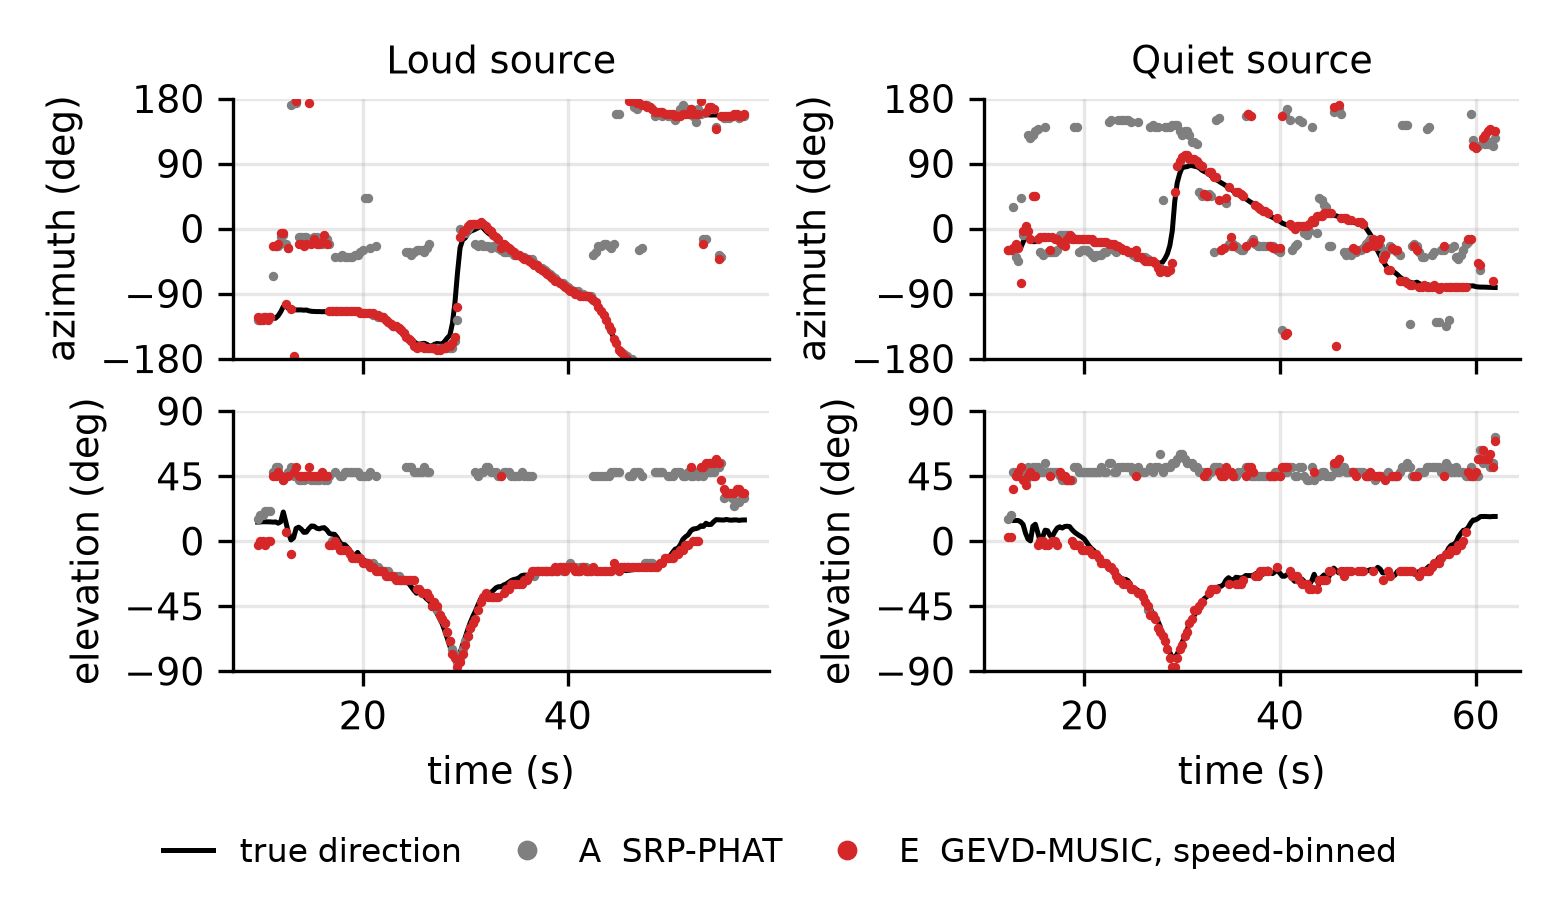
\includegraphics[width=0.82\textwidth]{fig/dregon_tracking.png}
\caption{True source direction (black) against the SRP-PHAT baseline (gray) and the speed-binned noise model (red) over two DREGON flights. The baseline locks onto the rotors at about $45$--$50^\circ$ elevation; the noise-model method follows the source through the maneuver.}
\label{fig:tracking}
\end{figure*}

\paragraph{Noise level.}
On clean recordings mixed with flight noise, all methods are accurate at 0 and $-5$\,dB.
At $-10$\,dB, D and E still localize 90\% of 48 trials within $10^\circ$, against 40--46\% for the others; at $-20$\,dB every method fails.
The noise model therefore buys about 5\,dB of operating range, but no method reaches the SNR at which distant calls for help would be heard.

\paragraph{Signal quality.}
Because a beamformer is linear, the target and the noise can be passed through it separately and the output SNR measured exactly.
Steering an MVDR beamformer (\cref{eq:mvdr}) with the learned covariance towards E's \emph{estimated} direction raises the SNR over a single microphone by a median of 9.7\,dB with speed-binned and 9.1\,dB with a single covariance, against 4.0\,dB for delay-and-sum, over 48 mixtures at $-10$\,dB input SNR.
\Cref{fig:snrfreq} shows that the gain is largest between 1 and 4\,kHz.

\begin{figure}[t]
\centering
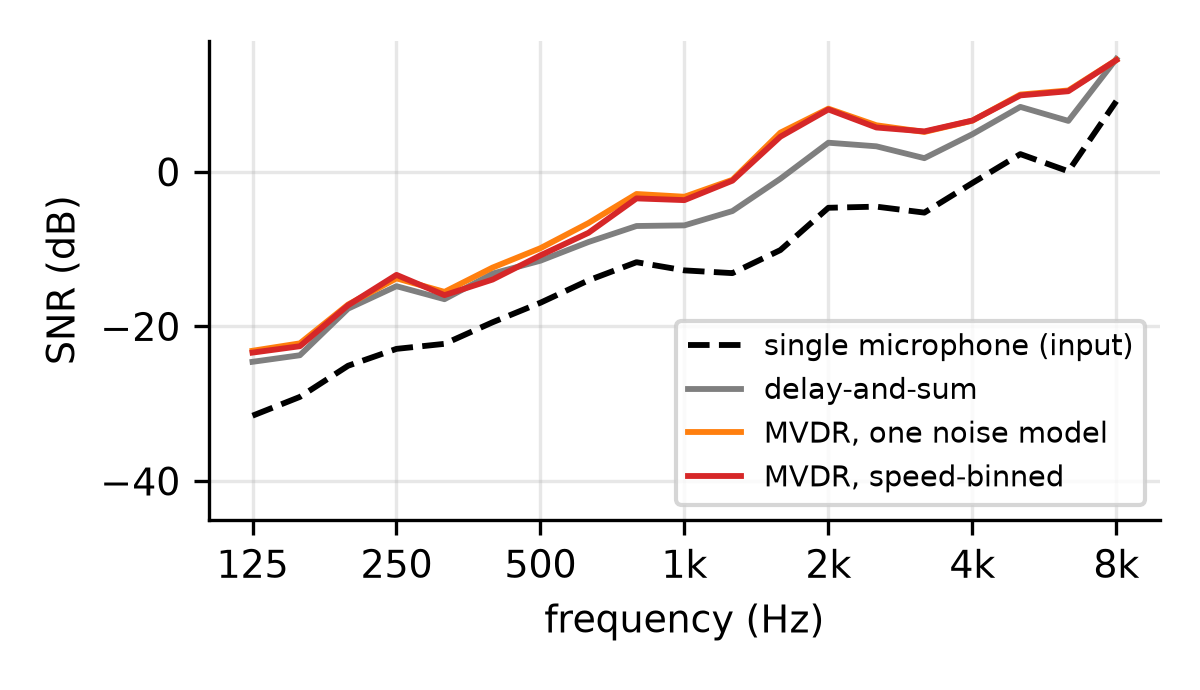
\includegraphics[width=\linewidth]{fig/dregon_snr_by_frequency.png}
\caption{SNR by third-octave band before (single microphone, dashed) and after beamforming towards the estimated direction, averaged over 48 mixtures at $-10$\,dB input SNR. A learned noise covariance (MVDR) roughly doubles the gain of plain delay-and-sum.}
\label{fig:snrfreq}
\end{figure}

\paragraph{Rotor tones and the IMU.}
Rotor tones are predictable from the motor log, but most of the noise energy on this drone is not on those tones.
The flight controller's IMU, sampled at about 1\,kHz, cannot observe vibration above 500\,Hz, which covers the lowest rotor harmonics (from about 140\,Hz) but not the band used for localization.

\subsection{Ego-noise across five drones}
\label{sec:case-drones}

A single drone cannot show whether these findings are general.
We therefore analyze noise-only recordings of four more quadrotors with 8-microphone arrays, released with the IEEE Signal Processing Cup 2019~\cite{deleforge2019spcup}: a DJI Phantom~4 Pro hovering outdoors at 2 and 10\,m, an MK Quadro~V3, an Intel Aero in manually controlled hover, and a quadrotor recorded at varying rotor speeds in an anechoic chamber (team AGH).
Of the other multichannel sets in that collection, two could no longer be downloaded, and one used a 16-microphone array whose published coordinates conflict with its photographs, so we did not use them.
Because the arrays differ, we use two measures that need no array geometry (\cref{fig:drones}).
The \emph{tonal share} is the share of 100--4000\,Hz noise energy in narrow spectral peaks, at least 6\,dB above a 300\,Hz running-median floor, computed on 1\,s chunks and averaged.
We define the \emph{learned rejection} to measure spatial structure.
It builds on the model of Wang and Cavallaro~\cite{wang2016earinthesky}, in which each rotor acts as one directional noise source and a diffuse part is added.
Because the microphones and motors are fixed to the frame, the acoustic mixing is stationary.
We learn the four strongest noise directions on the first half of a recording, one per rotor, and remove them from the second half with an orthogonal projection, as in the eigencanceler~\cite{haimovich1996eigencanceler}.
The learned rejection is the resulting drop in noise power, averaged over 300--4000\,Hz bins.
For the three arrays whose geometry was published, we compare it with a spherically diffuse noise field on the same array.

\begin{figure*}[t]
\centering
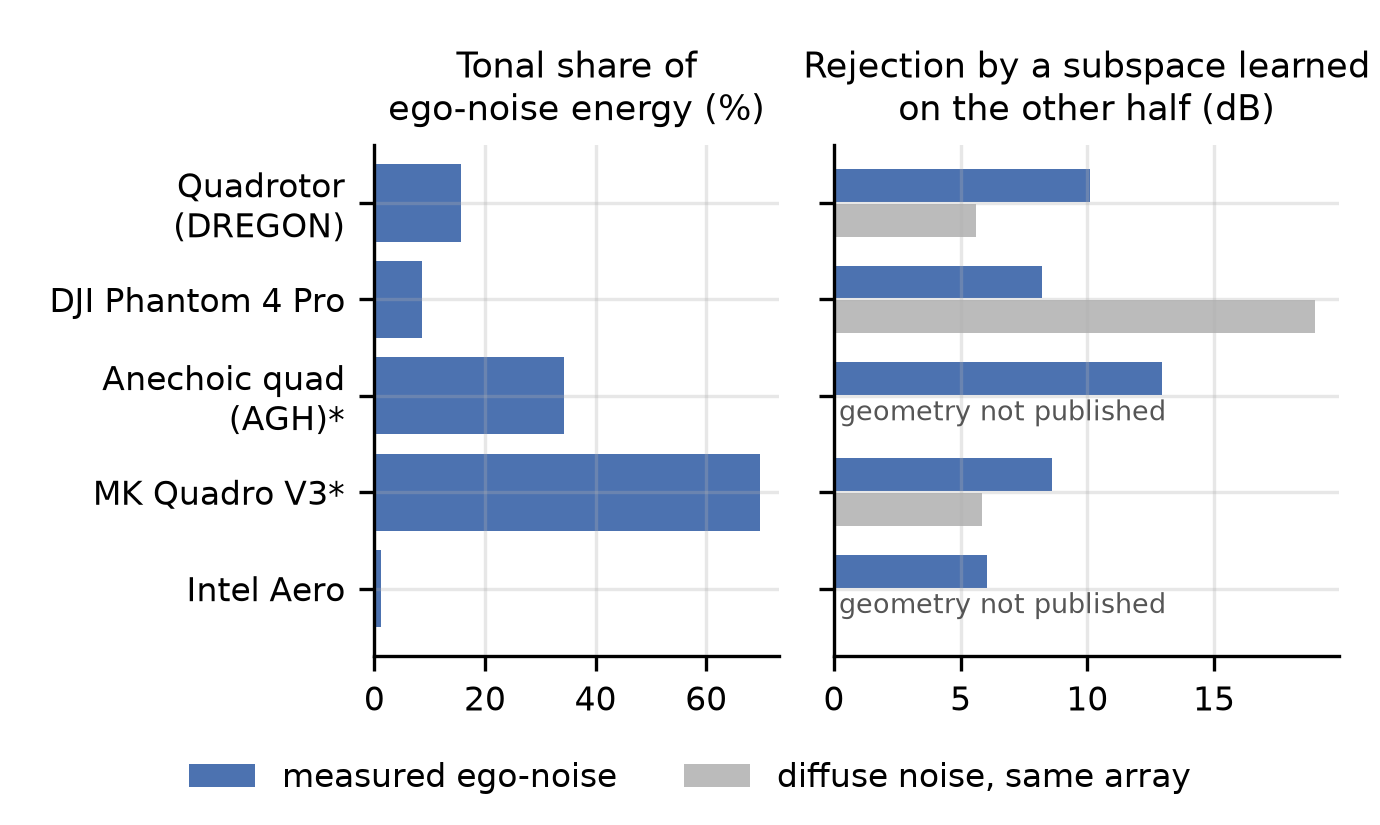
\includegraphics[width=0.68\textwidth]{fig/multidrone_egonoise.png}
\caption{Ego-noise of five quadrotors. Left: share of noise energy in rotor tones. Right: noise power removed from one half of a recording by a four-dimensional spatial subspace learned on the other half, against a diffuse noise field on the same array where the geometry is published. * represents a drone that was not flying during the recording. The MK Quadro~V3 was held about 0.5\,m above the floor. The AGH quadrotor stood still in an anechoic chamber.}
\label{fig:drones}
\end{figure*}

\paragraph{Results.}
Tonality differs by a factor of about 60 between drones: from 1\% of the noise energy (Intel Aero) through 16\% (DREGON) to 70\% (MK Quadro~V3).
However, the two highest values come from drones that were not in self-powered flight.
They are marked with an asterisk (*) in \cref{fig:drones}.
Among the three flying drones, the tonal share differs by a factor of about 13.
Masking or cancelling rotor tones is therefore valuable on some drones and nearly irrelevant on others.
A learned spatial subspace removes 6 to 13\,dB on every drone, and the model stays valid from one half of a recording to the other.
On the DREGON and MK Quadro~V3 arrays, with apertures of 17 and 15\,cm, it removes 4.5 and 2.7\,dB more than it would from diffuse noise, so the rotor noise is spatially more structured than background noise.
On the 6\,cm DJI Phantom array, however, a spatial model removes \emph{less} ego-noise than it would remove from diffuse noise (8.2 against 19.0\,dB).
This suggests that the noise is uncorrelated between the microphones.
Airflow over each microphone capsule may cause this.
Spatial models cannot remove such noise; larger apertures, flow shielding or single-channel suppression are needed instead.

\paragraph{Flight condition and tonality.}
In flight, the controller continually adjusts the rotor speeds.
This smears the rotor harmonics over each analysis window.
We measured the rotor-speed variation in each 1\,s window of the DREGON noise-only flight as the standard deviation of the logged speeds.
Windows with more variation have a lower tonal share (Spearman $\rho=-0.34$, $p=0.016$, 50 windows).
At the same mean rotor speed, their harmonic peaks are also lower (\cref{fig:jitter}).
Tonality measured on a drone that is not flying can therefore overstate the tonality in flight.

\begin{figure*}[t]
\centering
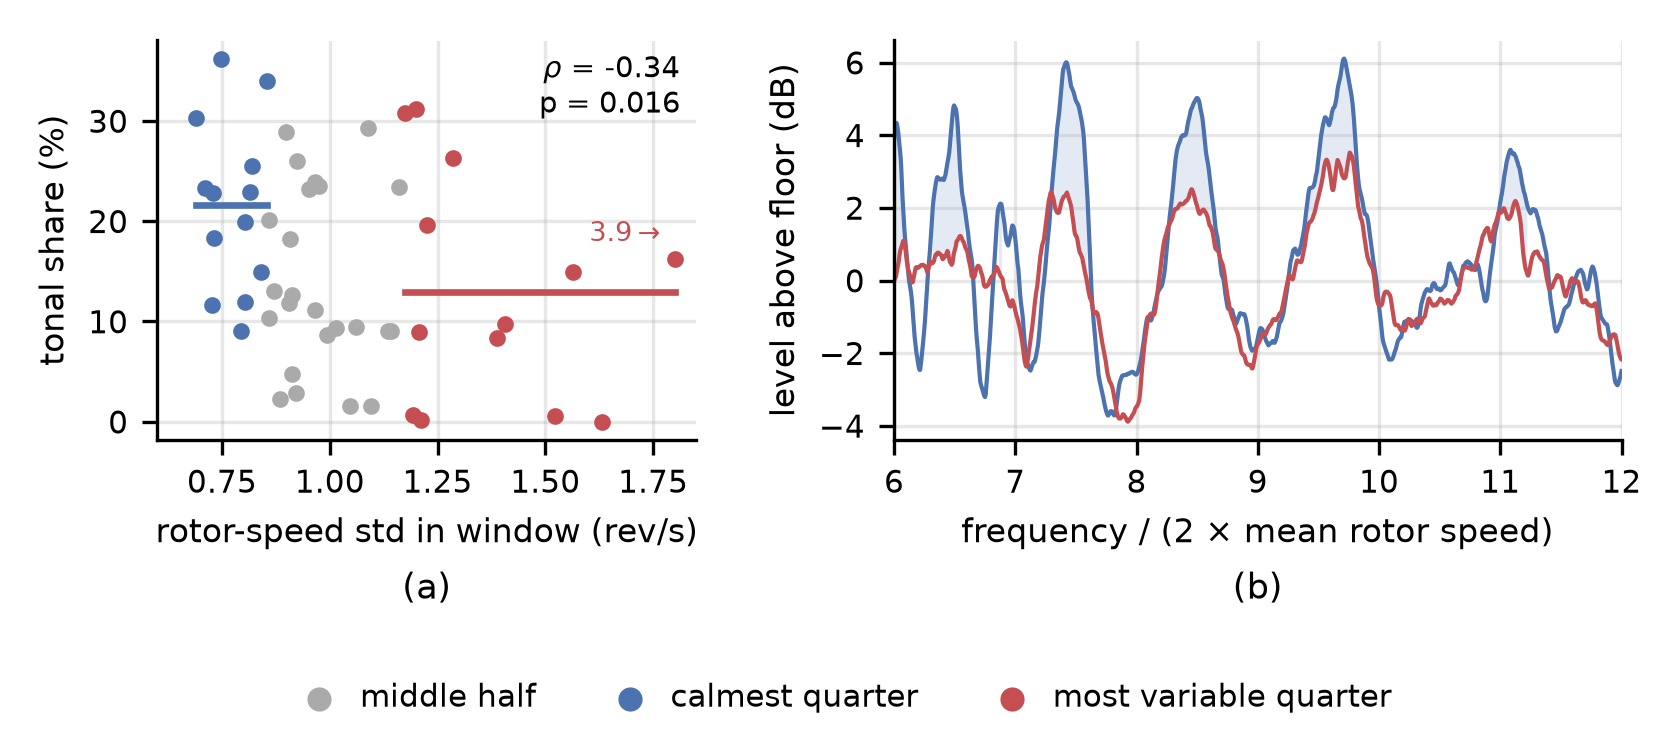
\includegraphics[width=0.78\textwidth]{fig/dregon_jitter_tonal.png}
\caption{Rotor-speed variation and tonal share in the DREGON noise-only flight (50 windows of 1\,s). (a) Tonal share against the standard deviation of the rotor speeds within each window. The standard deviation is averaged over the four rotors. Horizontal lines mark the mean of the calmest quarter (21.6\%) and of the most variable quarter (12.9\%). One window with 3.9\,rev/s is drawn at the edge. (b) Mean spectrum of these two quarters. Each window is aligned to its own mean rotor speed. Both quarters have the same mean speed (80.7 and 80.8\,rev/s). The harmonic peaks are lower in the variable windows (shaded).}
\label{fig:jitter}
\end{figure*}

\subsection{A robot-head array in a reverberant room (LOCATA)}
\label{sec:case-locata}

To test the localizers on a different platform and array, we use the robot-head array of the LOCATA development set~\cite{lollmann2018locata,evers2020locata}: a prototype NAO head with 12 microphones in a pseudo-spherical arrangement, recorded in a room with a reverberation time of about 0.5\,s, with optical tracking of the array and the sources and voice activity labels for every sample.
We use the three single-source tasks: a static loudspeaker with a static array (task~1), a moving talker with a static array (task~3), and a moving talker with a moving array (task~5).
The ground-truth direction is computed in the array's own frame from the tracked pose, so no alignment is fitted, and windows are scored when the source is active in at least 80\% of their samples (396 windows in total).
Methods B and E need motor speeds, which this platform lacks; method D learns its noise covariance from frames of the same recording in which the source is silent, at least 0.5\,s from any speech so that the reverberant tail does not leak in (or from all silent frames when fewer than 20 such frames exist).
The head has no running motors, so this study probes a regime without ego-noise.

\begin{table}[t]
\centering
\footnotesize
\setlength{\tabcolsep}{2.2pt}
\begin{tabular}{@{}lccc@{}}
\toprule
Method & Task 1 (34) & Task 3 (151) & Task 5 (211) \\
\midrule
A\; SRP-PHAT & 100\% / $4.8^\circ$ & \textbf{91.4\%} / $\mathbf{2.8^\circ}$ & \textbf{99.1\%} / $\mathbf{2.8^\circ}$ \\
C\; MUSIC & 100\% / $3.1^\circ$ & 86.1\% / $3.2^\circ$ & 95.7\% / $2.8^\circ$ \\
D\; GEVD, 0.5\,s guard & 100\% / $3.2^\circ$ & 69.5\% / $5.4^\circ$ & 68.2\% / $4.0^\circ$ \\
D\; GEVD, no guard & 100\% / $\mathbf{2.8^\circ}$ & 58.3\% / $8.0^\circ$ & 81.0\% / $4.6^\circ$ \\
\bottomrule
\end{tabular}
\caption{Localization with the LOCATA robot-head array: share of windows within $10^\circ$ / median angular error. Window counts in parentheses. Task 1: static loudspeaker and array; task 3: moving talker; task 5: moving talker and moving array.}
\label{tab:locata}
\end{table}

\paragraph{Results.}
\Cref{tab:locata} shows that the classical localizers are accurate on this array: SRP-PHAT places 91 to 100\% of windows within $10^\circ$, with median errors of 2.8 to $4.8^\circ$, also when both the talker and the array move.
The noise model does not help here; with moving talkers it lowers the share within $10^\circ$ by 18 to 33 points relative to SRP-PHAT, whether or not the reverberant tail is excluded.
The diagnostics explain why.
The SNR at the array is high, 16 to 25\,dB across recordings, and the background noise is close to diffuse: 75 to 89\% of its energy lies in the four strongest spatial components, against 79\% for a diffuse field on the same array.
There is little structured noise to remove, so whitening with a covariance estimated from a few hundred frames of changing background noise mainly distorts the spatial spectrum.

\subsection{What the case studies show}

Taken together, the three studies support a qualified version of the argument of \cref{sec:egonoise}.
\emph{(i)} When ego-noise dominates and is spatially structured, an explicit noise model is the largest single gain: on DREGON it raised in-flight accuracy within $10^\circ$ from 18\% to 70\%, and spatial noise models removed 6 to 13\,dB of ego-noise on all five drones.
\emph{(ii)} State information adds most when the target is weak: motor-speed-binned models gained 17 points over a single model on the quiet-source flight.
\emph{(iii)} The value of tone-based methods depends on the drone and on whether it is flying. Tonality ranged from 1\% to 70\% of the ego-noise energy, and rotor-speed variation in flight lowered it.
\emph{(iv)} A noise model is not free: when the SNR is high and the background close to diffuse, as on the robot head, it costs accuracy, so a system should decide from the measured noise conditions whether to apply it.
\emph{(v)} Array aperture and airflow limit what any spatial model can do, as the 6\,cm array showed.
All methods in these studies are established; the contribution is the controlled, reproducible comparison across platforms.

\section{Open Challenges and Research Directions}
\label{sec:challenges}

\paragraph{1. Hearing below $-15$\,dB.}
On drones, even noise-model methods fail between $-15$ and $-20$\,dB (\cref{sec:case-dregon}), yet distant calls for help fall in exactly this range.
Smooth, physically grounded noise models that vary with each rotor's speed~\cite{yen2023ncm}, combined with learned suppression~\cite{wang2022drone,gulli2025rotor}, are the most promising route.
Hybrid methods that first remove tones predicted from the motor state and then whiten the remaining spatial noise exploit complementary structure.
Longer integration windows help when the target is persistent, but conflict with the motion of the platform; tracking with motion compensation (direction 5) can bridge the two.

\paragraph{2. From masking to cancellation with vibration references.}
Motor state gives the frequencies of rotor and motor tones but not their phase.
A high-rate vibration sensor near each motor, combined with order tracking, could supply a phase-coherent reference and allow tones to be subtracted rather than masked.
Standard flight-controller IMUs are sampled too slowly for this (\cref{sec:case-dregon}), so dedicated sensors are needed; to our knowledge this direction is largely unexplored on autonomous platforms.
Its value depends on the drone: the tonal share of ego-noise ranged from 1\% to 70\% across the five drones of \cref{sec:case-drones}. Rotor-speed variation in flight also smears the tones. Tonality should therefore be measured in flight before tone cancellation is pursued.

\paragraph{3. Transfer across platforms.}
Ego-noise models are platform-specific, and learned models trained on one drone or robot rarely transfer.
Our multi-drone analysis suggests a starting point: on every drone, a spatial noise model learned from the first half of a recording of tens of seconds remained valid on the second half (\cref{sec:case-drones}), so short calibration flights may suffice.
Self-supervised adaptation from such recordings, and models conditioned on platform geometry and state rather than identity, would reduce the cost of deploying audition on a new platform.
Array design matters as much as the algorithm: on a 6\,cm array a spatial model removed less ego-noise than it would remove from diffuse noise.
Large pretrained audio encoders~\cite{kong2020panns,gong2021ast,chen2023beats} are a natural starting point if they can be made robust to ego-noise.

\paragraph{4. Simulation with ego-noise.}
Embodied simulators render room acoustics well~\cite{chen2022soundspaces2,gao2023sonicverse,luo2022naf} but omit the agent's own noise.
Adding parametric ego-noise driven by the simulated platform's state, calibrated on real recordings such as DREGON or AIRA-UAS~\cite{strauss2018dregon,ruizespitia2018aira}, would make sim-to-real transfer of audio-visual policies far more credible.

\paragraph{5. Temporal reasoning, active listening and confidence.}
A platform should also decide \emph{which} method to trust: in our studies a noise model was essential on a drone but cost accuracy on a quiet robot head (\cref{sec:case-locata}), so selecting or weighting methods from the measured SNR and noise structure is a practical first step.
Most localizers decide each short window independently.
Tracking with the platform's own motion compensated~\cite{valin2007tracking,evers2018slam,evers2020locata} and calibrated confidence from the sharpness of the spatial spectrum would let an agent know when it is wrong.
An agent that knows it is uncertain can also act to listen better, by moving~\cite{nakadai2000active,majumder2021move2hear} or, on a drone, by briefly changing its rotor speeds.

\paragraph{6. Open-vocabulary hearing.}
Audio-language models~\cite{elizalde2023clap,deshmukh2023pengi,gong2024ltu,tang2024salmonn} could let a platform report what it hears in words and search for sounds described in language.
Their robustness to ego-noise, their latency and their energy cost on embedded hardware have yet to be measured.

\paragraph{7. Benchmarks that match the problem.}
A shared benchmark with a moving platform, real ego-noise, platform state, high-rate vibration sensing, realistic intermittent sources (calls, whistles, speech) and video (\cref{sec:datasets}), evaluated with the protocols of \cref{sec:metrics} and archived with a persistent identifier, would align robot audition, drone audition and embodied learning around one problem.

\paragraph{8. Efficiency and energy.}
Few drone localization systems run in real time on board~\cite{chevtchenko2025review}.
Method papers should report computational cost on embedded hardware alongside accuracy, as lightweight localization work already does~\cite{grondin2019lightweight}.

\paragraph{9. Privacy and responsible use.}
Always-on microphones on robots, drones and vehicles can record people who have not consented.
Processing on board, keeping only the outputs a task needs (events and directions rather than raw audio), and suppressing speech content when it is not needed are practical safeguards that systems and benchmarks should support.

\section{Conclusion}
\label{sec:conclusion}

Acoustic perception gives autonomous systems a sense that reaches around corners and through occlusion, and the methods to exploit it, from array processing to large pretrained, audio-visual and language-grounded models, are increasingly mature.
What holds hearing back on real platforms is the platform itself.
This review has argued that ego-noise is the defining problem of the field, and that the platform's own knowledge of its state is the key to solving it.
Across robots and drones, methods that model ego-noise explicitly and use motor or joint data outperform those that treat it as generic interference when ego-noise dominates.
Our case studies on three public datasets quantify this: the advantage is largest exactly when the target is quietest, spatial noise models remove 6 to 13\,dB of ego-noise on all five drones studied, the value of tone-based methods varies widely between drones and flight conditions, and a noise model costs accuracy where there is little structured noise to remove.
Closing the remaining gap will require bringing together three communities that have so far worked largely apart: robot and drone audition, which understands ego-noise; audio machine learning, which provides robust representations; and embodied vision and learning, which provides the tasks, simulators and benchmarks that turn hearing into action.

{
    \small
    \bibliographystyle{ieeenat_fullname}
    \bibliography{main}
}

\end{document}
